% CAPITULO 1: EXPLICO EL ESQUEMA GENERAL DEL ALGORITMO

\chapter{Método/herramienta desarrollada}
\label{method}


\section{Fundamentos}
% Existencia de herramientas disponibles.
% Hipótesis asumida respecto del espacio de soluciones, dependencia de la superficie de búsqueda con las propiedades a evaluar.



Como se desarrollo a lo largo del capítulo 1, existen distintos elementos estructurales y funcionales que pueden estar presentes en una secuencia.
Clasificando, aislando y estudiando estos elementos podemos comprender mejor cuales son sus propiedades. 
Los avances en este campo se trasladan a una gran cantidad(y variedad) de métodos que permiten predecir la ocurrencia de las estas propiedades sobre una secuencia polipeptídica, tanto natural como artificial.
De forma abstracta, estas herramientas permiten predecir el mapeo entre la secuencia y el perfil de propiedades resultantes. 
% Diferentes herramientas bioinformáticas resultan de trasladar estos conocimientos a
% Estos avances, además, dieron paso al desarrollo de una gran cantidad(y variedad) de herramientas bioinformáticas que permiten predecir éstas propiedades a partir de la secuencia .
% La disponibilidad de estas herramientas permite tener una idea más clara del comportamiento que tendrá una proteína en un contexto experimental dado, solamente conociendo su secuencia y utilizando las herramientas adecuadas. 
% 


% COMPLEJIDAD DE LAS IDPs
% SACADO DE A decade and a half of protein intrinsic disorder: Biology still waits for physics
It was pointed out that IDPs possess noticeable amino acid biases, and many IDPs/IDPRs are characterized by sequence redundancy and low sequence
complexity, containing long stretches of various repeats and being completely devoid of some (often many) types of amino acid residues. 
These observations seem to indicate that the sequence space of IDPs/IDPRs should be simpler than that of ordered proteins.
However, the reality is more complex than conventional wisdom might suggest, and the sequence space attainable by simple IDPs/IDPRs is more diversified than that of the structurally more sophisticated ordered proteins.
In fact, a 100 residue-long protein in which any of the normally occurring 20 amino acids can be found has a sequence space of $20^100$ (aprox. $10^130$) sequences. 
Obviamente, no todas las secuencias al azar se pliegan para dar una estructura unica y, por lo tanto, no cualquier secuencia pertenecerá al conjunto que denominamos como plegadas.
In other words, a sequence space of a foldable protein (or “foldable” sequence space) is noticeably smaller than the entire sequence space available for a random polypeptide chain\cite{dill1999polymer}. 

Foldable proteins fold first and then bind to their partners whereas IDPs/IDPRs remain disordered until they interact with their partners. 
Furthermore, many IDPs/IDPRs do not require folding to be functional, and some of them form fuzzy complexes, in which they preserve significant amount of disorder. 
All this suggests that the sequence space of IDPs (at least those which either do not fold at all or do not completely fold at binding) 
is noticeably greater than the “foldable” sequence space due to the removal of restrictions posed by the need to gain ordered structure spontaneously. 
This represents one of the conundrums of intrinsic disorder, where the apparent sequence redundancy and simplicity are combined with the lack of structural restrains leading to the increase in the dimensions and complexity of the
available sequence space.


% 
% En los últimos años se han realizado importantes avances en el estudio de las relación existente entre la estructura primaria de proteínas y el conjunto de propiedades experimentalmente observables de éstas(\textit{in-vivo} o \textit{in-vitro}). 

% 
% 
% 
% El problema que estamos enfrentando es, sin embargo, el inverso. Queremos  
% Nuevamente, planteandolo de forma abstracta, esto representa mapear el espacio de comportamientos con el espacio de secuencias posibles.
% 
% Claramente, ambos problemas están íntimamente relacionados: un mejor entendimiento de los principios que hacen posible(y necesarios) para que una secuencia tenga un cierto comportamiento, brindarán mayor información
% It is clear that the two problems are closely related to each other: a better understanding of the principles of protein folding makes it possible to clarify which features of protein sequences are necessary (as well as sufficient) 
% for stability and fast folding; in other words, the features that make a protein a protein. 
% Such understanding focuses the attention of designers on emphasizing these crucial features of folding sequences.
% 
% Obtener una secuencia con un comportamiento muy específico(por ejemplo que adquiera una estructura plegada definida), puede ser un requerimiento muy específico.
% Un reflejo de esto puede verse en las estructuras de ciertas proteinas naturales, las cuales tienen una fuerte dependencia con la secuencia que se mantiene altamente conservada. 
% 
% Sin embargo, como se detalló en la sección previa, el objetivo de nuestra herramienta es lograr obtener una secuencia con un comportamiento bastante 'simple' de obtener.... 



De esta forma, estamos en una situación en la que: tenemos un conjunto de herramientas que nos permiten mapear cada secuencia con distintos comportamientos (deseado o no deseados) de acuerdo a nuestro objetivo y, además, 
podemos asumir que el conjunto de secuencias que cumple con los principales comportamientos buscados, es considerablemente grande dentro del espacio de secuencias posibles (cualquier combinación de AAs).

El esquema de búsqueda dependerá de nuestros objetivos y los conocimientos, desconocimientos, hipotesis acerca del espacio de búsqueda.
Una primera aproximación obvia sería probar distintas combinaciones al azar...
El problema es que es una forma totalmente ineficiente de búsqueda, tiene un alto costo computacional y el resultado(asumiendo que lo encontramos) tendrá una composición al azar(esto puede no resultar un problema, dependiendo del objetivo especifico).

Una aproximación mas adecuada sería utilizar todo el conocimiento que tenemos acerca de la evaluación de la secuencia. 
La existencia de una función ideal implicaría que esta represente la dependencia de cada posicion con el contexto de la secuencia, con respecto a la propiedad analizada.
Si bien las herramientas disponibles de predicción nos son las ideales, generalmente brindan información sobre cada posición y no sobre la secuencia como un todo.

Uilizando esta información podríamos analizar que posiciones no son acordes con el comportamiento/propiedades deseado/a y utilizar esta información para guiar la búsqueda, modificando solo aquellas posiciones que no nos resultan favorables.
 
Si bien asumimos que el conjunto de secuencia que cumplen las condiciones estandar del resultado es grande con respecto al especio total de soluciones, no conocemos la forma funcional que no esta guiando la busqueda,
es decir, como esta depende con la secuencia.  Para implementar un mecanismo eficiente de búsqueda debemos tener en cuenta este desconocimiento.




\section{Esquema general de la implementación}




\subsection{Secuencia inicial}

El método comienza la búsqueda a partir de una secuencia inicial. 
Esta secuencia puede ser creada de forma aleatoria como primer paso del algoritmo(ver \ref{secuenciaInicialRandom}) o puede ser pasada como parámetro por el usuario \ref{secuenciaInicialDefinida}. 

La generación de una secuencia aleatoria no es un problema trivial. 
En la naturaleza las proteínas están compuestas de un conjunto de 20 aminoácidos, los cuales se encuentran con diferentes abundancias relativas. 
La frecuencia de cada aminoácido dentro de un proteoma está dada por un balance entre el costo metabólico de este y la necesidad de contar con un conjunto de secuencias diversas que darán proteínas funcionales \cite{krick2014amino}. 
Para generar una secuencia aleatoria, entonces, es necesario definir la frecuencia que tendrá cada aminoácido. 
Esta frecuencia se obtiene a partir de la frecuencia global que tiene cada aminoácido en la base de datos de secuencias proteicas.
La aplicación que se utiliza para obtener la secuencia random es RandSeq \cite{randseq}.

Por default, la herramienta utiliza la composición estándar obtenida de SwissProt \cite{compositionAA}.  
Estos valores resultan del cálculo de la composición de aminoácidos de todas las proteínas de la base de datos. 
De esta forma, la composición total representa un consenso de frecuencias de aminoácidos entre todas las secuencias documentadas hasta el momento en la base de datos UniProtKB/Swiss-Prot.
% Los valores de la composición estándar se encuentran en http://web.expasy.org/protscale/pscale/A.A.Swiss-Prot.html

Entre otras que existen, esta herramienta ofrece la posibilidad al usuario de definir las frecuencias que desea para cada aminoácido e, incluso,
indicar solo la frecuencia de algunos residuos en particular, dejando el restos con la frecuencia estándar. 
Nuestra herramienta también ofrece al usuario esta flexibilidad para definir la composición que tendrá la secuencia (ver \ref{composicion})
Esta funcionalidad permitiría, por ejemplo, indicar que cierto aminoácido no esté presente en la secuencia (asignándole una frecuencia igual a 0). 
Para el fin que tiene la herramienta, es útil tener este tipo de funcionalidades ya que permite adaptar los requerimientos a las capacidades(limitaciones) del laboratorio experimental. 
El nuevo linker diseñado deberá poder ser sintetizado eficientemente junto con la nueva proteína, lo cual implica una carga metabólica para el sistema biológico en el cual está siendo producido. 
De esta forma, se intentará adaptar las propiedades de la secuencia diseñada para aumentar la capacidad de síntesis reduciendo, por ejemplo, los aminoácidos que implican un gran gasto energético y que limitarán la producción de la proteína final.




\subsection{Método de evaluación de la secuencia}


% Para poder implementar la busqueda guiada por información resultante de evaluaciones secuenciales, primero debemos poder representar esta información de forma concreta/cuantitativa.
% Para esto, de cada evaluación realizada sobre la secuencia se extrae un valor binario para cada posición. Un valor = 1 representa una evaluación negativa con respecto al comportamiento deseado, 
% mientras que un valor = 0 implica una evaluación positiva.
% Por ej: .........
% ARMAR EJEMPLOS CON HERRAMIENTAS SIN ESPECIFICAR EL NOMBRE DE ESTA,ej:  LA EVALUACION DE LA HERRAMIENTA A RESULTA EN..... Y LA HERRAMIENTA B RESULTA EN ...
% Los valores correspondientes a distintas
% Por ej. si al analisis previo le agregamos una evaluacion para....

% Usando este esquema, se deduce simplemente que la posicion que tenga el mayor valor será la que mas se aleja de nuestro objetivo.

% Una de las desventajas(quizás no), de este esquema , es que el metodo esta orientado a realizar evaluaciones que permitan derivar un valor binario para cada posicion de la secuencia. 
% Esto, al parecer, no seria un problema, ya que el resultado deberia poder adaptarse a este esquema.


% Ya que no conocemos la función exacta que determina la relacion entre la secuencia y los valores de puntajes en las distintas posiciones(ni tampoco su superficie funcional),
% no podemos conocer como varía el puntaje asociado si realizamos una modificacion sobre la secuencia
% Ademas, esta variacion del puntaje con la secuencia depende de distintos factores, no solo del conjunto de herramientas/evaluaciones realizadas, sino también de los parámetros utilizados para éstas.
% La implementación de la búsqueda deberá tener esto en cuenta para realizar una busqueda guiada por estos valores.





\subsection{Búsqueda heurística/guiada}



% La implementación realizada sigue un esquema conocido como método de Monte Carlo. 
% Para guiar la búsqueda se utilizará el valor global del puntaje asociado a la secuencia. Este valor resulta de la suma 
% La posición a mutar mutación 



% TENIENDO EN CUENTA ESTAS CONSIDERACIONES, EL ESQUEMA QUE USAMOS NOS PERMITE REALIZAR UN NUMERO REDUCIDO DE MUTACIONES YA QUE SE APUNTA A LAS POSICIONES CON MAS CONFLICTO, 
% ADEMAS EL PARAMETRO BETA PERMITE ADAPTAR LA BUSQEUDA A DISTINTAS FORMAS DE LA SUPERFICIE DEL ESPACIO DE SOLUCIONES, LAS CUAL DEPENDE DE LAS CONDICIONES DE LOS PARAMETROS QUE USAMOS(COMPOSICION, THRESHOLDS, HERRAMIENTAS).
% ES DECIR SI LA SUPERFICIE TIENE MINIMOS LOCALES QUE DEBAN SER SUPERADOS, UN VALOR DE BETA MAS ALTO RELAJA LAS RESTRICCIONES PARA
% ACEPTAR MUTACIONES Y POR LO TANTO PERMITE . CUANDO LA SUPERFICIE ES MAS 'PLANA', UN VALOR DE BETA MENOR PERMITE ENCONTRAR LA SOLUCION CON UN MENOR NUMERO DE MUTACIONES(LO QUE NO SIGNIFICA QUE SEA MAS RAPIDO)
% En este caso, la función a optimizar está dada por el resultado de todas las evaluaciones que queremos realizar.


% Una particularidad de este problema es que, si bien no conocemos su forma funcional(dependencia de la secuencia con las características de comportamiento que ) ni podemos resolver el problema del su valor mínimo() 
% tenemos cierta información acerca de la imágen de esta función, o al menos del valor al cual queremos llegar.
% El uso de un método probabilistico apunta a mejorar la performance en la búsqueda de la solución pero también aporta propiedades no deterministas al algoritmo.


El procedimiento general del algoritmo consiste en iterar sobre la secuencia inicial, evaluando en cada paso las propiedades de cada posición de la secuencia con respecto a características de interés. 
Los resultados de cada evaluación serán reflejados en un valor numérico o puntuación asociado a cada posición. En cada iteración el puntaje es inicializado en 0 para todas las posiciones y cada evaluación ejecutada puede aumentar o mantener el valor, de manera tal que, al finalizar todas las evaluaciones correspondientes a una iteración, el puntaje de cada posición tendrá un valor mayor o igual a cero. 
El aumento de este puntaje depende de la concordancia que tiene cada posición con las características evaluadas. En cada evaluación se aumenta el valor si el residuo en esa posición NO favorece la propiedad deseada.
Al terminar todas las evaluaciones de cada iteración, el puntaje resultante se utiliza para decidir si es necesario realizar una mutación puntual sobre la secuencia y, de ser así, sobre que posición se realiza.
PONER EJEMPLO PARA QUE QUEDE CLARO

El proceso de mutación se realiza al final de cada iteración y consta de dos pasos:
    -En primer lugar se selecciona uno de los residuos de la secuencia como objetivo para realizar la mutación. Esta selección será ponderada, utilizando como factor de ponderación el puntaje asociado a cada posición. Se debe tener en cuenta que, como se mencionó previamente, el valor del puntaje resultante puede ser igual a 0 y, si esto se repite para todas las posiciones, puede ocurrir que ningún residuo sea factible de ser seleccionado, en cuyo caso no se continúa el proceso de mutación. 
    -El segundo paso, asumiendo que algún residuo fue seleccionado, consiste en seleccionar con que aminoácido se sustituirá éste. Esta selección se realiza siguiendo la misma distribución que se utilizó para generar la secuencia inicial. Dado que la selección del sustituto es independiente del tipo de residuo seleccionado para mutar, es posible que el mutado y su reemplazo seleccionado sean iguales. En este caso simplemente se vuelve a seleccionar un sustituto hasta que el resultado sea un residuo distinto al anterior.     

    -El tercer paso consiste en aceptar o rechazar la mutación según un algoritmo de Monte Carlo. Para realizar esto se vuelve a evaluar el puntaje, analizando todas las características deseadas de la secuencia pero, esta vez, el análisis se hará sobre la secuencia que contiene la mutación propuesta, la cual se aceptará si el puntaje asociado es menor que el  resultante de la secuencia sin la mutación incorporada. De forma resumida, solo se incorporan mutaciones que se traduzcan en una disminución del puntaje total de la secuencia.
En caso de no aceptarse la mutación propuesta el algoritmo vuelve al primer paso del proceso de mutación.

El algoritmo busca, en cada iteración, reducir el puntaje de la secuencia introduciendo una mutación. Dado que el objetivo final es obtener una secuencia que posea, con cierta probabilidad, todas las características deseadas, el algoritmo finaliza cuando el puntaje resultante sea igual a cero. Esto implica que todas las evaluaciones concuerdan con los objetivos buscados en el diseño de la secuencia linker.


% DIBUJAR DIAGRAMA DE FLUJO O PSEUDOCODIGO DEL ALGORITMO
En la figura \ref{fig:esquema-algoritmo} se ve un esquema general del método, aplicado al problema de secuencias que queremos tratar.



\begin{figure}[htbp]
\centering
   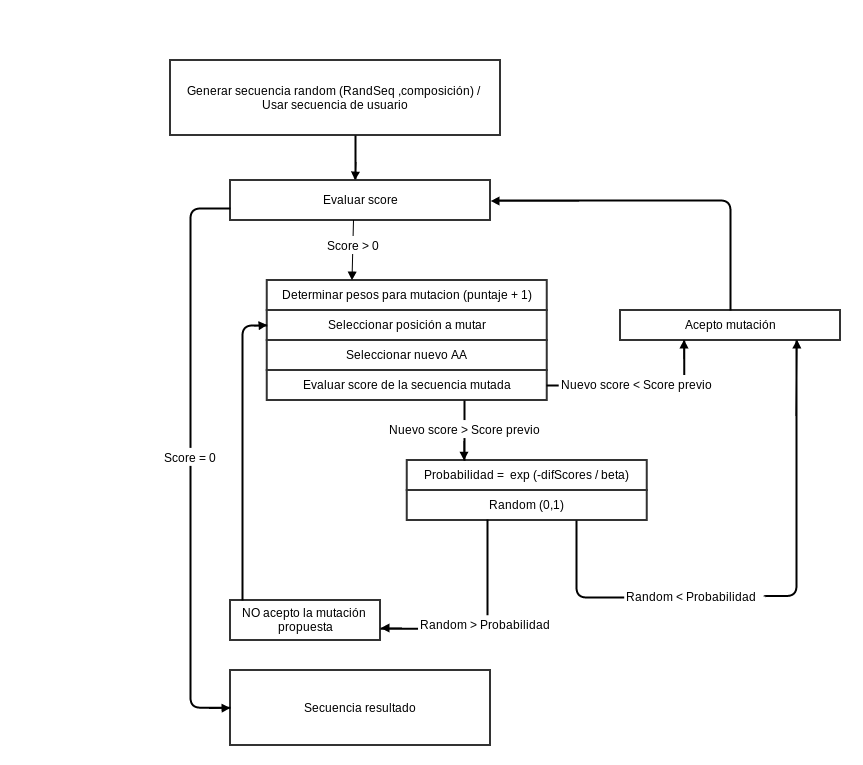
\includegraphics[width=\textwidth]{img/diagrama-algoritmo.png}
 \caption{Esquema general del método aplicado para obtener la secuencia final}
 \label{fig:esquema-algoritmo}
\end{figure}



\subsubsection{Método de mutación}
% POR QUE HACEMOS UNA MUTACION DE A 1 PASO, ES DECIR 1 SOLA MUTACION POR VEZ? 

